% begin Chapter ResearchMethodology

\chapter{Research Methodology}
\label{chapter-ResearchMethodology}

\paragraph{ } In Chapter~\ref{chapter-LitReview} we discussed the theoretical basis of scheduling and the planning process of a public transport system. We also analyzed the current literature related to the various stages of the planning process (i.e.:timetabling, vehicle and crew scheduling and crew rostering). Furthermore, in Chapter~\ref{chapter-Introduction} we discussed the background of the present system and the problems associated with the current bus scheduling process as well as the bus transport system as a whole. This chapter will detail the research methodology that was followed during this research project.

The main research objective was to find a solution to help all the stakeholders involved in the public transportation system. In order to do so, people in the scheduling process of the transport system as well authoritative persons in charge of regulating the service were interviewed. In particular, the \acrshort{ntc} and the \acrshort{wp} \acrshort{rpta} was contacted and several relevant people were interviewed to understand the system \& the service and to ascertain the current problems of the system. A list of persons interviewed have been noted below.

\begin{itemize}
\item Mr. Pradeep Fernando - Head of the \acrshort{gps} Tracking and Monitoring Unit, \acrshort{ntc}.
\item Mr. Dhanushka - Team Member, \acrshort{gps} Tracking and Monitoring Unit, \acrshort{ntc}.
\item Mr. Muditha Navaratne - Timetable Unit of the \acrshort{ntc}.
\item Mr. K.A.R.A. Ranjith - Operations Manager, \acrshort{wp} \acrshort{rpta}.
\item Mr. Mahesh Nishan - Scheduling Officer, \acrshort{wp} \acrshort{rpta}.
\item Mr. Theja Athukorala - Scheduling Officer, \acrshort{wp} \acrshort{rpta}.
\item Mr. M. T. L. Cooray - Training Officer, \acrshort{wp} \acrshort{rpta}.
\item Mr. Janaka Weerawardana, doctoral candidate at the University of Moratuwa, Department of Transport and Logistics Management.
\item Mr. Anuradha Piyadasa, a Consultant and an Academic in the field of Public Transportation and Management.
\end{itemize}

After the interviews were carried out, a better understanding of the transportation system's workings and its issues began to emerge. It was then that a pilot route survey was conducted. Details of the survey is mentioned in the following section.



\section{Pilot Route Survey}

\paragraph{ } The bus route chosen for the study is the 177 bus route that runs between Kolpetty and Kaduwela. The route segment between Kolpetty and Rajagiriya was taken into consideration when collecting the data. It is a high value route and is graded as "A+" in a scale of A+, A, B, C by the \acrshort{wp} \acrshort{rpta} based on the passenger demand and importance of the route. Additionally, it has buses that are consistently overcrowded and commuters complain about it frequently. Buses on the route are also prone to loitering and many complaints are received regarding this issue making it a perfect candidate to carry out the pilot route survey.

There are 49 buses in in the normal fleet in total with 35 in daily operation. All buses have the capacity to carry around 45 passengers (seated) on average. The route also has Air Conditioned (AC) buses but we will not be considering the AC buses in our data gathering.

\subsection{Data Gathering Methodology}

\paragraph{ } Data was collected by physically traveling in the bus at various times and manually counting the number of passengers that get on and off the bus. This provided information about the passenger demand and load situations in the bus. The time at which the bus arrives and departs each bus stop was also observed and recorded. The time spent at each bus stop was calculated using this data. If the bus loitered at a certain bus stop, the amount of time the driver spent loitering was also recorded.

The data was gathered in this manual way because there is no automated data gathering mechanism currently in place for the private bus system in the Western Province. As mentioned previously, the current data gathering is done manually by the schedulers at the \acrshort{wp} \acrshort{rpta}. The implementation of an \acrshort{adcs} has not been carried out yet due to the reasons mentioned in Chapter~\ref{chapter-LitReview}. Therefore, the problem remains, how can the data be collected in order to aid in the scheduling and timetabling activities of the \acrshort{rpta}.

The data that is required for the schedulers is the Vehicle Location data and the Passenger Demand data. The former could be obtained by using just a few \acrshort{gps} tracking devices such as the ones the \acrshort{ntc} uses in their system, which are fixed temporarily to a few buses. The problem the schedulers face currently is that they have to physically travel in the buses to collect the data. Alternatively, they could use a few (~5-10) devices to temporarily track the selected buses for the purposes of the survey freeing the need for the schedulers to travel in the buses physically themselves and gather the data. The devices don't have to be fixed permanently onto the buses, just when the survey is being conducted so that the data can be gathered on its movements.

Gathering of the Passenger Demand data is a little more trickier. Passenger Demand is basically a reflection of the number of people that travel in a bus and details of where they get on and off the bus. This could be achieved by counting the number of tickets issued and analyzing the ticketing data. This method however, has a major drawback. It assumes that all commuters are issued a ticket which may not always be the case. Also, not all buses currently have Electronic Ticketing Machines which is an obstacle. The fact that it is not compulsory for the private buses in the \acrshort{wp} plying on intra-provincial routes to have Electronic Ticketing Machines is also a major disadvantage to this method. In conclusion, it is clearly evident that reform and stricter regulation of the service is required in order to improve it.

Section~\ref{GatheredData} displays a sample of the data that was gathered during the pilot route survey. The data confirms what most commuters complain about on a regular basis, that the bus loitering is a problem that needs to be dealt with. The survey data also implied that loitering adds to the problem of overcrowding buses which results in increased dissatisfaction by the commuters.

\subsection {Gathered Data}
\label {GatheredData}

\paragraph{ } Listed below is a sample of the data that was collected. The full list of data is available under Appendix~\ref{appendix-CompleteSetOfData}.

\paragraph{Trip Number: 1}
\begin{itemize}
\item Date: 23/5/2013
\item Departure Time: 15.40pm
\item Departure Place: Kolpetty
\item Tables~\ref{table-trip1-BoardingAndAlighting} and~\ref{table-trip1-LoiterTime}
\end{itemize}

\begin{table}[H]
\centering
\begin{tabular}{|l|r|r|r|r|}
\hline
Bus Stop & Boarded & Alighted & Net Gain & On Board \\
\hline
 & & & & 0 \\
Kolpetty Depot	&11	&0	&11	&11\\
Supermarket	&10	&0	&10	&21\\
Alwis Place	&7	&0	&7	&28\\
Library	&3	&6	&-3	&25\\
SLTA	&0	&2	&-2	&23\\
\rowcolor[gray]{0.7}
Museum	&1	&0	&1	&24\\
Nelum Pokuna	&2	&2	&0	&24\\
\rowcolor[gray]{0.7}
Alexandra Roundabout	&5	&0	&5	&29\\
Asha Central	&2	&1	&1	&30\\
Wijerama	&4	&0	&4	&34\\
Borella	&2	&5	&-3	&31\\
Devi Balika	&1	&1	&0	&31\\
Castle Street	&1	&0	&1	&32\\
Ayurveda	&2	&6	&-4	&28\\
Rajagiriya	&25	&5	&20	&48\\
\hline
\end{tabular}
\caption{Boarding And Alighting data for Trip 1}
\label{table-trip1-BoardingAndAlighting}
\end{table}

\paragraph{} The fields highlighted in grey in Table~\ref{table-trip1-BoardingAndAlighting} signifies the places where the bus dropped off and picked up passengers where there was no designated bus stop. As is evident, there are passengers who get on and off the bus at undesignated stops. This also occurs because bus drivers stop at those places allowing passengers to board and alight the bus.

%\begin{landscape}
\begin {figure} [H]
\centering
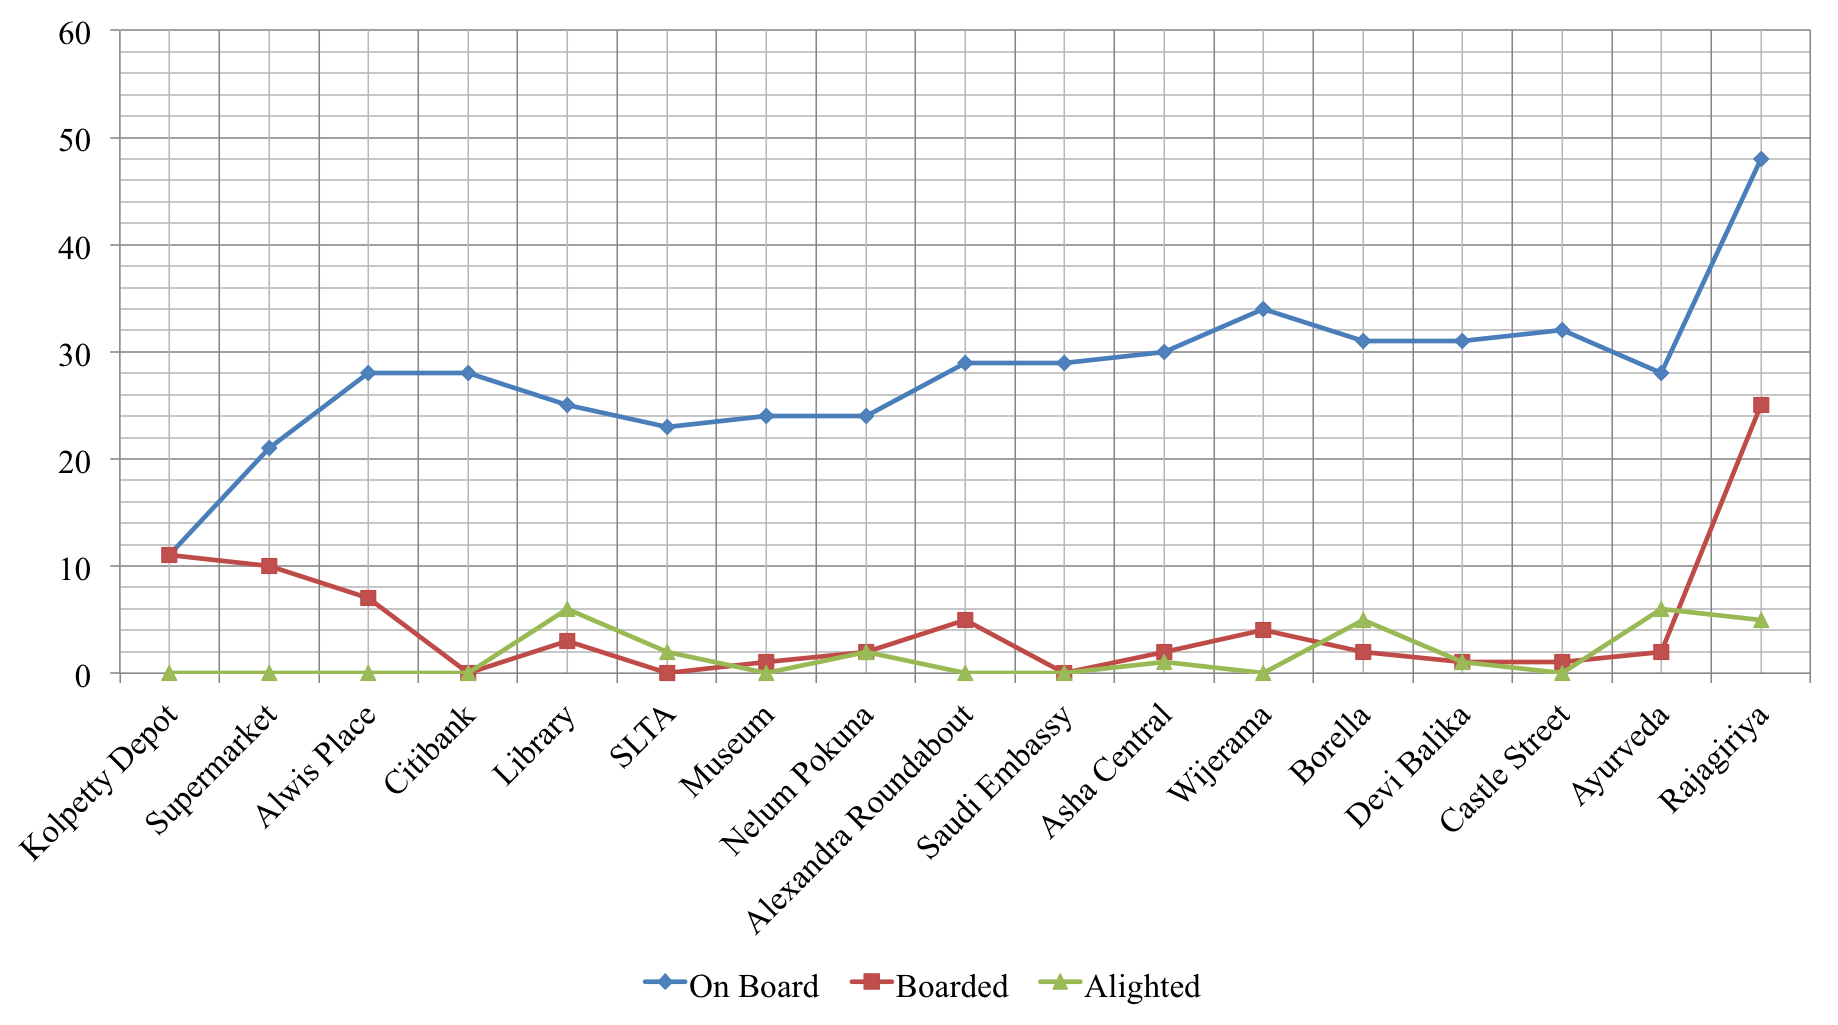
\includegraphics[scale=0.5]{passengerLoadData-Trip1}
\caption [Graph - Passenger Load Fluctuations - Trip 1] {Graph - Passenger Load Fluctuations - Trip 1}
\label {image-passengerLoadData-Trip1}
\end {figure}
%\end{landscape}

\paragraph{} Figure~\ref{image-passengerLoadData-Trip1} shows a graphical description of how the passenger load fluctuated throughout the trip. The trip started from the Kolpetty Depot (where the 177 bus route commences its operation) and ended at the Rajagiriya bus stop (The service on the route continues on after Rajagiriya). The red line on the graph depicts the number of passengers who boarded the bus at each stop while the green line depicts the number of passengers who alighted the bus at each stop. The sum of these 2 graphs shows the number of people in the bus at any given moment, which is depicted by the blue line on the graph. As you can see from the graph, after the initial influx of passengers boarding the bus at the Kolpetty depot, there is a fairly consistent inflow of passengers boarding the bus as well as an outflow of passengers alighting the bus. This means that the number of passengers on the bus at any given time on average is a constant. However, there is a sharp increase in passengers boarding the bus at Rajagiriya. This is caused by the loitering of the bus at the Rajagiriya bus stop. 

\begin{table}[H]
\centering
\begin{tabular}{|l|r|r|r|}
\hline
Bus Stop & Arrival Time (h) & Departure Time (h) & Loiter Time (mins) \\
\hline
Kolpetty Depot	&	&15.40	&0\\
Supermarket	&15.44	&15.45	&1\\
Alwis Place	&15.46	&15.46	&0\\
Library	&15.48	&15.49	&1\\
SLTA	&15.50	&15.51	&1\\
Nelum Pokuna	&15.52	&15.53	&1\\
Asha Central	&15.56	&15.56	&0\\
Wijerama	&15.58	&15.58	&0\\
Borella	&16.08	&16.09	&1\\
Devi Balika	&16.11	&16.11	&0\\
Castle Street	&16.14	&16.14	&0\\
Ayurveda	&16.15	&16.16	&1\\
Rajagiriya	&16.18	&16.24	&6\\
\hline
Total Loiter Time & & & 12 mins \\
Duration of Trip & & 44 mins & \\
\hline
\end{tabular}
\caption{Loiter Time Data for Trip 1}
\label{table-trip1-LoiterTime}
\end{table}

\paragraph{} Table~\ref{table-trip1-LoiterTime} details the time the bus spent loitering at each stop during the trip under consideration. The Arrival Time and the Departure Time columns depict time stamps (accurate to the minute) at which the bus arrived at or departed from a given bus stop. Total Loiter time is the sum of the individual loiter times at each stop. Duration of the trip is calculated by substracting the departure time at Rajagiriya from the departure time at the Kolpetty depot. As the data shows, 12 out of the 44 minutes of this trip was wasted on loitering at bus stops, a 27.27\% wastage of time for both the commuters as well as the bus operators.

%\begin{landscape}
\begin {figure} [H]
\centering
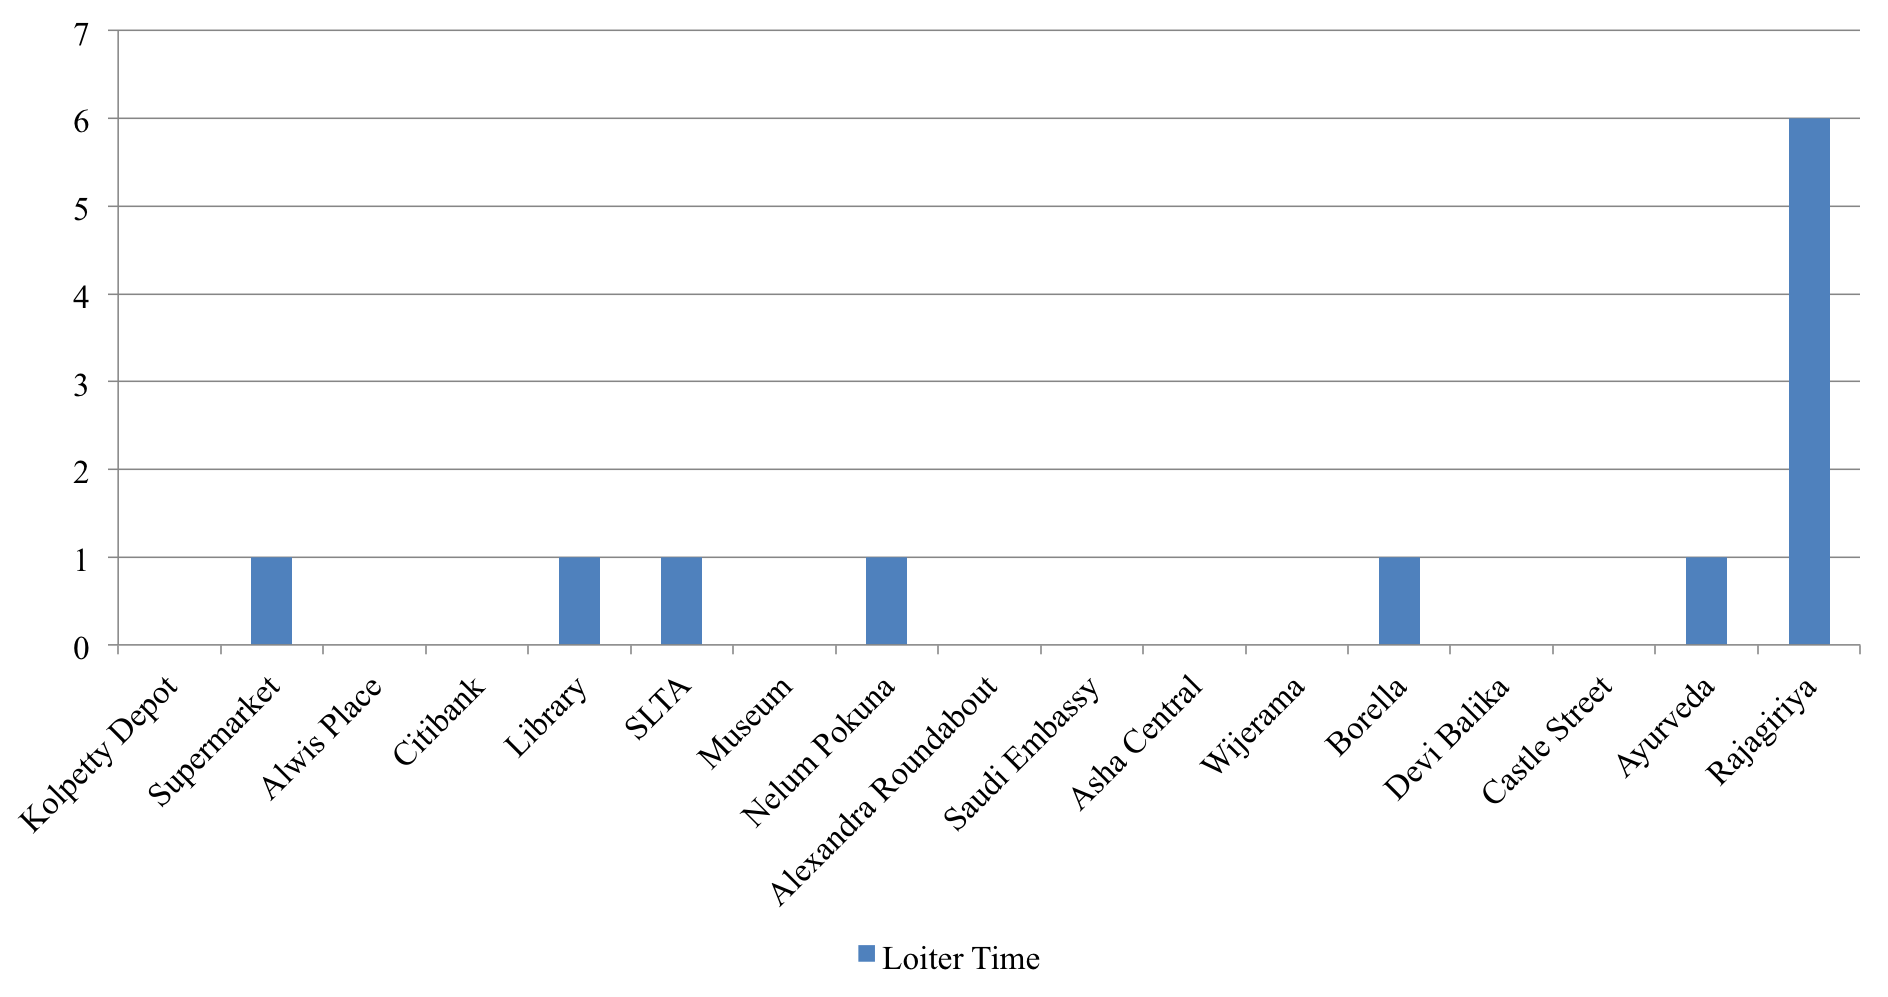
\includegraphics[scale=0.5]{loiterTimeData-Trip1}
\caption [Graph - Bus Loiter Time Data - Trip 1] {Graph - Bus Loiter Time Data - Trip 1}
\label {image-loiterTimeData-Trip1}
\end {figure}
%\end{landscape}

\paragraph{} As Figure~\ref{image-loiterTimeData-Trip1} clearly illustrates, the bus loiters for a considerable period of time at the Rajagiriya bus stop. This leads to an overcrowded bus when it leaves the Rajagiriya bus stop as corroborated by Figure~\ref{image-passengerLoadData-Trip1}. The loitering results in the discomfort of existing passsngers as well as the ones that are expected to board the bus at the bus stops later on in the route.



\section {Stakeholder Analysis}
\label {StakeholderAnalysis}

\paragraph{} Research observations together with interviews conducted with the personnel at the \acrshort{ntc} \& the \acrshort{wp} \acrshort{rpta} have shown that there are 5 main stakeholders in this Public Transport System and they are illustrated in Figure~\ref{image-stakeholdersDiagram}. As any information system needs to correctly identify its stakeholders first, information was gathered through interviews with several people in the \acrshort{wp} \acrshort{rpta} as well as the \acrshort{ntc} \cite{Mahesh2013a, Theja2013a, Mahesh2013b, Navaratne2013a, Navaratne2013b,  Ranjith2013a, Weerawardena2013, Piyadasa2013}. Futher information was garnered through personal experience, interviews with frequent commuters of the bus service and the pilot route survey (detailed earlier in this chapter) \cite{Bandara2013, Pallegoda2013, DeSilva2013, Senevirathne2013}. The "government" and "other motorists" are minor stakeholders pertaining to this system and although has no direct impact on the bus service, is affected by what happens to it and therefore has been included in this consideration.

\begin {figure} [H]
\centering
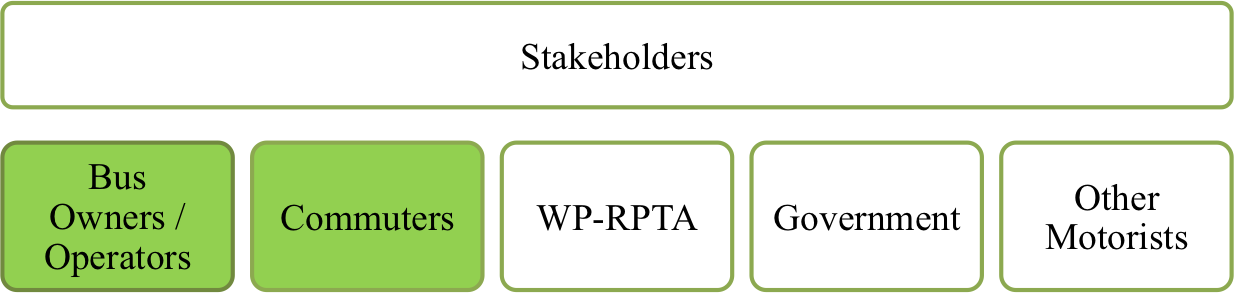
\includegraphics[scale=0.75]{stakeholdersDiagram}
\caption [Stakeholders Diagram] {Stakeholders Diagram}
\label {image-stakeholdersDiagram}
\end {figure}

\paragraph{} The most prominent stakeholders in this system are the Commuters and the Bus Owners/Operators (shaded in green circles). These 2 serve as the demand and supply sides of the economic equation respectively. Although they have conflicting requirements, these two parties are essential to the proper functioning of the system. The \acrshort{wp} \acrshort{rpta} is the other major stakeholder in this system. It is the Transport Authority's responsibility to keep the two main parties happy and provide a satisfactory service to the public. Therefore, the most important stakeholder of the whole system is the Transport Authority and that is why it is important that an information system is implemented that assists the schedulers in their decision-making process. 

\begin {figure} [H]
\centering
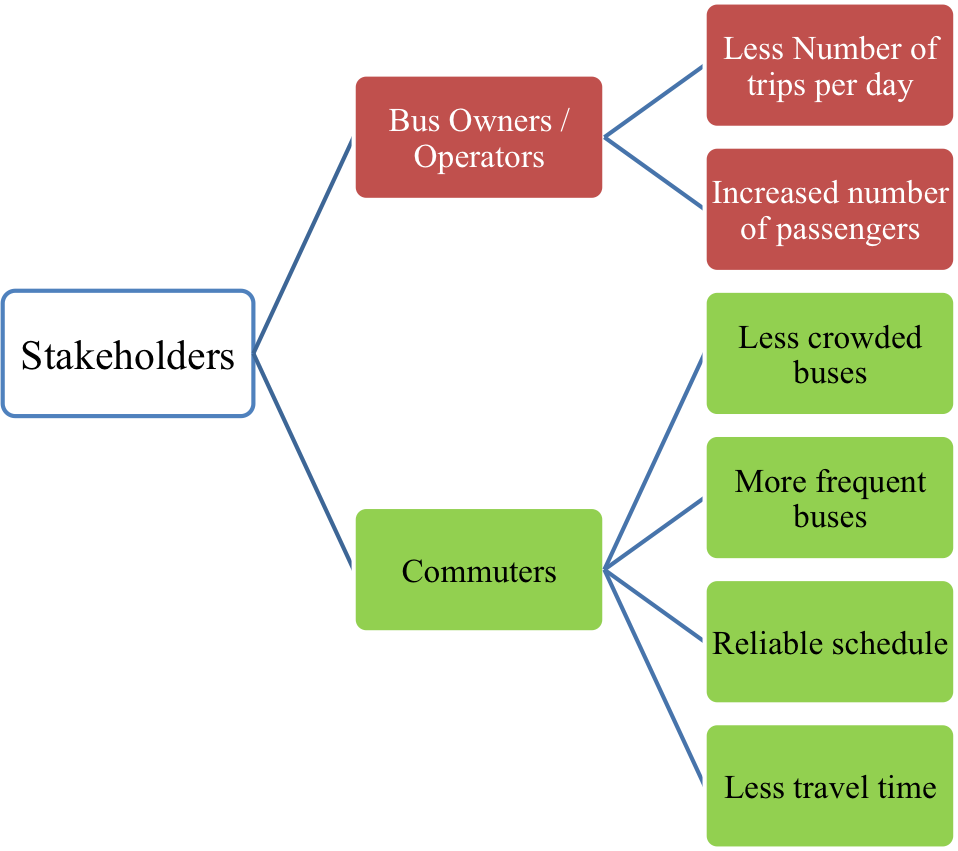
\includegraphics[scale=0.8]{mainStakeholdersDiagram}
\caption [Requirements of Main Stakeholders] {Requirements of Main Stakeholders}
\label {image-mainStakeholdersDiagram}
\end {figure}

\paragraph{} The conflicting requirements of the bus owners/operators and the commuters have been highlighted in Figure~\ref{image-mainStakeholdersDiagram} \cite{Mahesh2013a, Theja2013a, Mahesh2013b, Navaratne2013a, Navaratne2013b,  Ranjith2013a, Weerawardena2013, Piyadasa2013}. As is illustrated, The commuters require a more comfortable journey, whereas the main concern for the bus operators is the revenue generation by any and all means.

The workflow of the Scheduling Unit of the \acrshort{wp} \acrshort{rpta} is comprised of 3 main stages  \cite{Mahesh2013a, Theja2013a, Mahesh2013b, Ranjith2013a, Piyadasa2013}. They are illustrated in Figure~\ref{image-timetablingProcessSteps}. Gaman, the prototype Decision Support System detailed in Chapter~\ref{chapter-SolutionPrototype}, will contain this workflow at its core. Further information regardin this process has been given in Section~\ref{section-CurrentBusSchedulingProcessInSriLanka} previously in this document.

\begin {figure} [H]
\centering
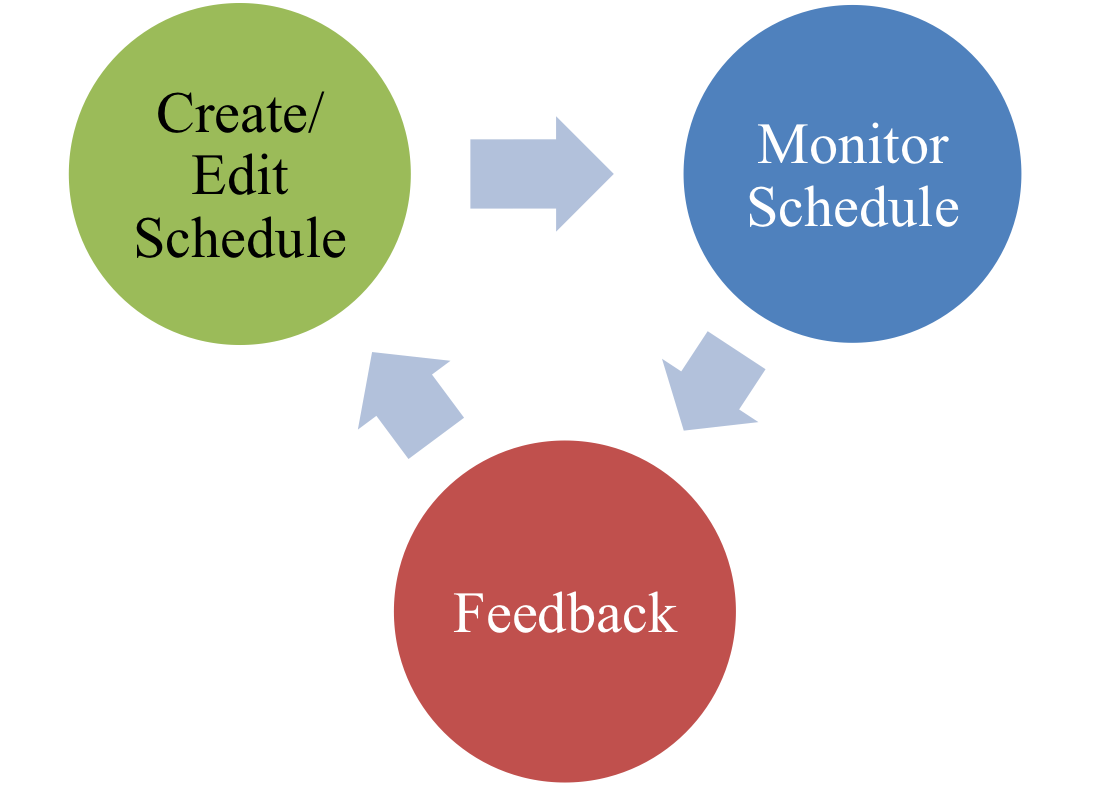
\includegraphics[scale=0.7]{timetablingProcessSteps}
\caption [Stages in the Timetabling Process Flow] {Stages in the Timetabling Process Flow}
\label {image-timetablingProcessSteps}
\end {figure}

The definition of a \acrshort{dss} and how it relates to the transportation problem has already been discussed in this document. Therefore, in the next Chapter, we will see what the proposed solution is. This will include the higher-level system architecture, the system features, the main entities \& their relationships and a few UI screenshots of the prototype that was built for user testing.



\section{Evaluation of Alternatives}

\paragraph{} Next in the research methodology, an evaluation of the alternative options is provided. It has already been established that an information systems solution closely resembling a \acrshort{dss} is required to cater to the problems existing in the current transportation system. Therefore let us take a look at some existing software available on the market today.

Considering existing software solutions, there are a few scheduling software solutions available in the market right now but all of them offer products that cater to more modern, structured and developed transportation systems \cite{Trapeze2013a}. The cost associated with these systems is also very high.

For instance GIRO’s HASTUS software is an integrated solution that provides modules for transportation planning, scheduling, operations, passenger information, and analysis. HASTUS is designed for all modes of public transportation – from bus and BRT busway, to metro, heavy rail, and commuter rail \cite{GIRO2013}.

CTS-Software Inc. is another software vendor that produces scheduling, dispatching, billing, and reporting software for public transit companies. Their Trip Master Enterprise Edition (TMEE) software provides a platform that a Transportation Agencies can use for the aforementioned steps in the planning and management process (CTS Software Inc., 2013).

Other software vendors also exist but as previously mentioned they do not cater to developing countries and their requirements. The cost factor associated with advanced software such as this is also a hurdle in purchasing and implementing a similar system in a developing country like Sri Lanka \cite{Trapeze2013b}.

Therefore, we see that existing systems don't quite fulfill the requirements of the current problem. A system that is suitable for deployment in a developing country where there is little infrastructure of gathering data automatically and where cost is a major issue is what is needed. Unfortunately there is no such system currently available on the market. Please refer to Figure~\ref{image-FeasibilityMatrix} for an illustration of the feasibility of the available options.

\begin {figure} [H]
\centering
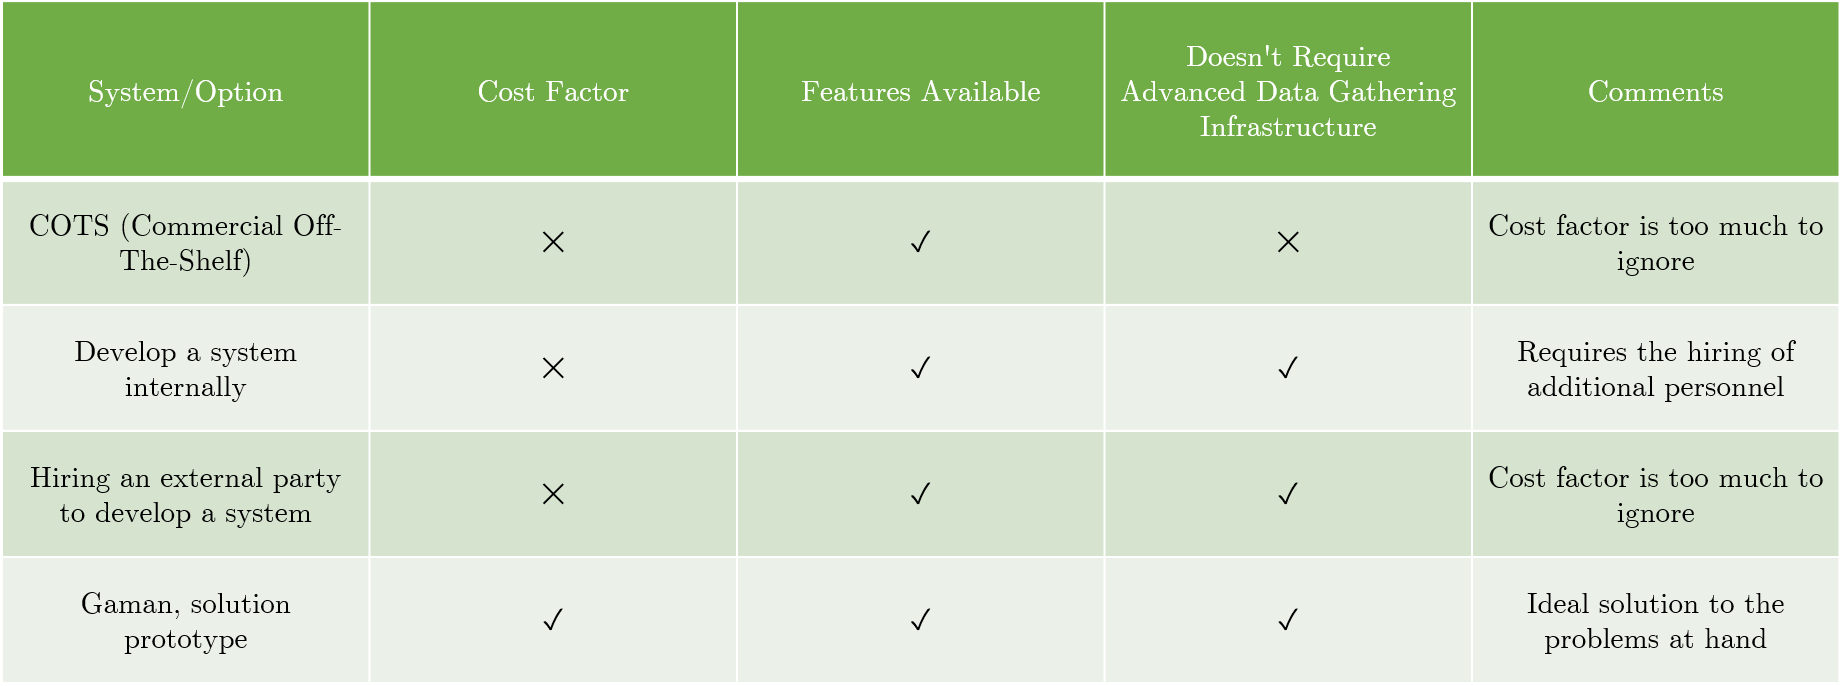
\includegraphics[scale=0.5]{feasibilityMatrix}
\caption [Feasibility Matrix of Alternative Systems/Options] {Feasibility Matrix of Alternative Systems/Options}
\label{image-FeasibilityMatrix}
\end {figure}

The focus of the research consequently moves to building a prototype information system that fulfills the aforementioned requirements. The prototype was then tested with commuters and the schedulers at the transport authority. Further details of the solution prototype and the evaluation are given in Chapters~\ref{chapter-SolutionPrototype} and ~\ref{chapter-ResearchEvaluation} respectively. Since the type of information system that is needed has already been established in Section~\ref{section-possibleISSolution} the research moves directly to the building of the prototype and evaluating it with the users.

So far in the document we have seen the problems existing in the public bus transport system. It was also shown that the issues required an information system to solve the problems and aid the stakeholders in their decision making process. An analysis of which type of \acrshort{is} is required was also prvided. Consequently, the relevant literature regarding the planning process of a typical public transport system was documented. Next, the topic of Automatic Data Gathering was addressed and details of how it relates to the planning process were given. The research methodology that was followed during the project was detailed in this chapter. Therefore, in the next chapter we will take a look at Gaman, the solution prototype that was built for the purpose of this research project. The next chapter will provide an in-depth look at the solution prototype, it's features and some UI screenshots.









